\subsection{projecting and image using K* [I | O]}

\begin{figure}[H]
\centering
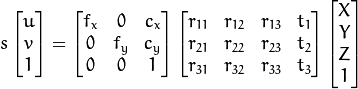
\includegraphics{pics/homogenious_projection.png}
\label{homogenious_projection}
\end{figure}

When we want to project 3d coordinates to the 2d image plane we multiply the
coord vector by K * [I | O] matrixes and converts the result to
homogeneous coords on the 2d image plane. Here (X,Y,Z) is the world
coordinate and (U,V) is the image coordinate. 
The column vectors [r1, r2, r3] of the “I” extrinsic matrix represent the
directions of the world-axes in camera coordinates.
